\section{What the correction acts on}
\label{sec:leverage}

Section~\ref{sec:intervention} shows the projection helps and that a random law of the same
complexity hurts, which says the effect is specific without saying what it is specific \emph{to}.
This section measures that. For each direction $u$ in the extracted subspace we record its
statistical prominence and its causal leverage,
\begin{equation}
V(u) = \operatorname{Var}(u^\top z), \qquad
D_H(u) = \mathbb{E}\bigl[L_H(z + \epsilon u) - L_H(z)\bigr],
\end{equation}
where $L_H$ is the model's own $H$-step rollout error. $V$ is what principal-component analysis
reports. $D_H$ is what the model's dynamics say the direction is worth, and it needs no simulator.

\paragraph{Errors compound rather than decay.} A displacement injected into the latent grows as the
model rolls forward. After 40 steps it retains $6.3\times$ its initial size at $\epsilon = 0.05|z|$,
$2.8\times$ at $\epsilon = 0.25|z|$ and $1.9\times$ at $\epsilon = 0.5|z|$, as medians over the three
seeds; larger displacements amplify less, as a saturating nonlinearity does. A contracting transition
would make small latent errors self-correcting and this whole section moot. This one amplifies them,
which is why a bounded invariant error turns into an unbounded trajectory error.

\paragraph{Calibrating the displacement.} Our first attempt used $\epsilon = 0.05|z|$ and produced
damage near $-0.5\%$ of baseline with the sign varying between directions, which read as ``variance
predicts consequence at $+0.40$''. The rollout is exactly deterministic, so a repeated unperturbed
rollout differs by zero and those values were not sampling noise: $\epsilon$ was too small for the
response to leave the second-order regime. Damage against displacement for the leading direction runs
$-0.5\%$, $+3.1\%$, $+18.1\%$, $+46.4\%$, $+128.8\%$ at $\epsilon/|z|$ of $0.05$, $0.10$, $0.25$,
$0.50$, $1.00$. We fix $\epsilon = 0.25|z|$, the smallest displacement whose damage exceeds $10\%$ of
baseline while the response still grows smoothly.

\begin{figure}[t]
\centering
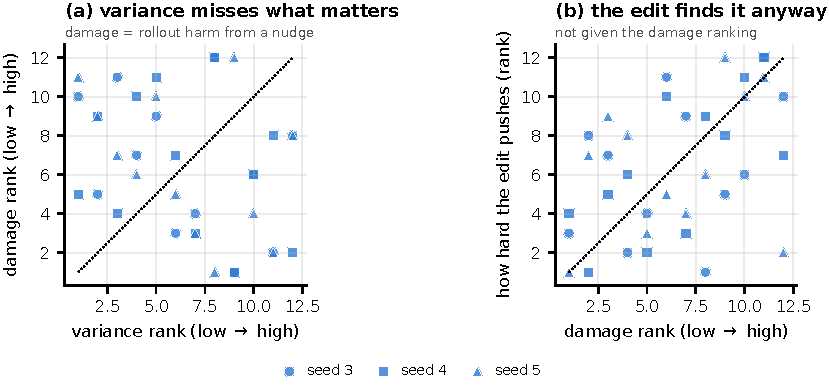
\includegraphics[width=\textwidth]{figures/fig4_leverage.pdf}
\caption{Each point is one of the twelve extracted directions, ranked within its own model; the
dotted line marks perfect agreement. \textbf{(a)} The directions the latent gives the most variance
are not the ones a nudge hurts most, on any seed (rank correlation $-0.36$, $-0.26$, $-0.41$ for
seeds 3, 4, 5). \textbf{(b)} The projection of Section~\ref{sec:intervention} nonetheless pushes
hardest on exactly those high-damage directions ($+0.38$, $+0.69$, $+0.29$), though the correlation
is far from perfect, so the correction is only partly targeted.}
\label{fig:leverage}
\end{figure}

\paragraph{The edit acts on the directions that matter.} How hard the projection pushes on each
direction correlates with $D_H$ at $+0.385$, $+0.692$ and $+0.287$ across seeds, positive on all
three (Figure~\ref{fig:leverage}b). The correction spends its effort where displacement does the most
damage. The correlation sits well short of $1$, so the correction is partly targeted and partly
spread across the latent.

\paragraph{Variance misses those directions, at short horizons.} At the same 40-step horizon,
prominence and damage anti-correlate: $-0.364$, $-0.259$, $-0.406$, negative on all three seeds, with
damage spanning $13.5\times$ to $118.8\times$ between the most and least consequential direction
(Figure~\ref{fig:leverage}a).

We checked whether that survives a change of horizon before drawing anything from it, and it does not
survive far. Rank correlation of $D_H$ between disjoint halves of the evaluation trajectories is
$0.95$, so the per-direction measurement itself replicates. The disagreement with variance does not:

\begin{center}\small
\begin{tabular}{lccc}
\toprule
horizon & 20 & 50 & 100 \\
\midrule
median $\rho(V, D_H)$ & $-0.252$ & $-0.196$ & $-0.028$ \\
negative in & \textbf{9/9} settings & 5/9 & 5/9 \\
\bottomrule
\end{tabular}
\end{center}

At horizon 20 the anti-correlation holds for every seed and every displacement we tried. By horizon
100 it is gone, and one seed reaches $+0.727$. The explanation is simple: once a rollout has diverged
from the truth, whichever directions carry the most amplitude dominate the total error, so variance
and damage measure the same thing. The mismatch lives in the regime where the model still tracks the
system.

\paragraph{What we have not established about it.} Everything in this section measures
the conservative models alone, so we cannot say whether the mismatch is a property of a model
that learned a conserved quantity or of autoregressive prediction on smooth data generally.
Separating those needs the same measurement on a matched model with no conserved quantity. We
have that model (the dissipative arm of Section~\ref{sec:refusal}) and report the
comparison as future work rather than folding an unreviewed result into this claim.

\paragraph{The correction reproduces functionally, but not coordinate-wise.} Three models trained
identically except for their seed agree closely on everything we can state without reference to a
basis, and disagree on everything we cannot. Recovery agrees to $0.008$, the edit's dose-response
slope to $0.016$, and the curvature of the gradient field, measured as the top-3 eigenvalue mass of
$M_C = \mathbb{E}[gg^\top/\|g\|^2]$, to $0.046$ ($0.448$, $0.441$, $0.487$).

Now select a protected subspace two ways and score each by the same dose-response slope. Ranking the
latent \emph{coordinates} by $\nabla C$ and keeping the top three gives $-0.075$, $+0.016$, $-0.089$:
it beats a variance ranking on two seeds of three, loses badly on the third, and changes sign, so it
fails a margin we had registered on all three. Replacing the coordinate mask with an orthogonal
projector onto the top eigenspace of $M_C$ beats the variance selector on all three seeds. The
coordinate-dependent selector varies by $0.105$ across seeds where the basis-free quantities vary by
$0.008$ to $0.047$; those are different quantities on different scales, so the comparison is
suggestive rather than decisive, but the sign change is not a matter of scale.

We take that to mean the models implement the same physical structure in different internal charts.
One limit on the subspace result, stated because it is easy to overread: on two seeds the gradient
subspace also sits below the 5th percentile of a hundred random rank-3 subspaces, but on the third
it sits at the 41st. It is better than variance on every seed and not yet shown to be better than an
arbitrary subspace of the same rank.

That $M_C$ has less than half its mass in three of twelve directions is worth stating on its own.
The correction is rank one at every state, so this spectrum measures how much $\nabla C$
\emph{rotates} as the state moves. It rotates a lot, and by the same amount in every model. The
law-bearing direction curves through the latent instead of resting on a fixed set of axes.

\paragraph{Takeaway.} The projection that improves rollouts acts on directions whose displacement
damages the model's own predictions, and at short horizons those are not the directions the latent
makes prominent. Read together with the paragraph above, the practical lesson is that the
reproducible object here is a function of the state, not a coordinate: asking which latent units
carry the physics gives a different answer in every model, while asking which direction the recovered
law points in gives the same one. We report this as a caution for coordinate-level readings of a
learned latent, and note the limit of our own evidence: comparing subspaces \emph{across} models is
not well defined in raw latent coordinates, since each model's basis is arbitrary, so what we show is
agreement of basis-free scalars rather than coincidence of the subspaces themselves. We state this as a measurement rather than a design principle: the effect is weak,
it decays with horizon, and we have not shown that a model built to protect high-damage state
predicts better than one built to protect high-variance state. That comparison is what would turn
this into an architecture, and we have not run it.
